% =============================================================================
% Solar Filament Segmentation Challenge 2026 -- technical report
% Yuxuan Li.  Content built on the official competition template
% (main.tex / preamble.tex / main.bib).  Guide text removed; \guideStylefalse.
% =============================================================================
\documentclass[sigconf]{acmart}
\input{preamble}

% Guide styling: \guideStyletrue = show gray italic hints; \guideStylefalse = omit them
\guideStylefalse

\begin{document}

\title{Solar Filament Instance Segmentation with a Lightweight YOLO11-seg Baseline}
\subtitle{A Solution to the Solar Filament Segmentation Challenge 2026}

\author{Yuxuan Li}
\affiliation{%
  \institution{Xi'an Jiaotong-Liverpool University}
  \city{Suzhou}
  \country{China}
}
\email{yuxuan.li2304@gmail.com}

\begin{abstract}
This report describes our solution to the Solar Filament Segmentation Challenge~2026, a Kaggle competition on automatic segmentation of solar filaments in GONG H-$\alpha$ observations.
We fine-tune a stock \texttt{yolo11n-seg} model at $1024\times1024$ on the MAGFiLO annotations, using an annotator-aware COCO-to-YOLO conversion, a month-grouped train/validation split, and an RLE post-processing stage that enforces the competition's non-overlapping-mask rule.
On the held-out month (174 distinct frames, 2094 annotated filaments) we measure mean Dice $0.640$ and global PQ $0.2845$; raising the confidence threshold from $0.10$ to $0.25$ moved our public score from $0.21$ to $0.25$.
We report three ablations, the three instance-level distributions required by the rubric, and a measurement of how strongly PQ depends on the ground-truth protocol ($0.2622$--$0.2816$).
\end{abstract}

\maketitle

\ifguideStyle
\noindent{\color{gray!65}\itshape Guide mode is on.}
\par\medskip
\fi

% ====================================
% INTRODUCTION
% ====================================
\section{Introduction}
This report goes over the details of our submitted solution to the Solar Filament Segmentation Challenge~2026 \cite{filament-segmentation-2026}. The challenge, launched on July~10,~2026, is organized by the Earth-Space AI Research (ESAIR) Lab\footnote{\href{https://www.esairlab.com/home}{www.esairlab.com/}}. This challenge utilizes the MAGFiLO dataset for evaluation of the segmentation algorithms \cite{ahmadzadeh2024dataset}.

Our architecture is deliberately left unmodified: we use an off-the-shelf YOLO11-seg model, so that every difference we measure is attributable to data handling or inference settings rather than to network design. We make four contributions. (i)~Input resolution is the only training knob we found that moves PQ materially. (ii)~Doubling the training budget is a negative result: every detection metric improves while PQ does not. (iii)~Using the three instance-level distributions the rubric requests, we identify the mechanism by which \emph{halving} the number of predictions improved our public score. (iv)~We bound the evaluation's own uncertainty by re-scoring one fixed set of predictions under four ground-truth protocols.

% ====================================
% METHODOLOGY
% ====================================
\section{Methodology}\label{sec:methodology}

\subsection{Data and sampling strategy}
The organisers provide MAGFiLO \cite{ahmadzadeh2024dataset} as a COCO annotation file plus $2048\times2048$ 8-bit \emph{grayscale} H$\alpha$ JPEGs. Each COCO image entry carries $2048\times2048$ polygons, one per filament, with \texttt{iscrowd}$=0$ throughout. The first thing worth reporting is the structure of the file: its $1154$ image entries map to only $\mathbf{707}$ \textbf{distinct files}. The \texttt{id} field concatenates an annotator batch with the file name (\texttt{010401-20160920230134Lh}), and each frame was annotated independently by up to three of the $\sim\!40$ annotators. Crucially, the annotators produced \emph{complementary partial} sets of filaments rather than duplicates of one another --- a fact that, as Section~\ref{sec:evaluation} shows, changes how the ground truth should be assembled.

Two design decisions follow. First, a random split would place the \emph{same physical frame} in both training and validation, and neighbouring solar frames are near-identical, so the leak would be severe. We therefore split by whole calendar months, holding out one month in every four (\texttt{VAL\_EVERY}$=4$; 29 of 118 months). Second, we never key exported labels on \texttt{file\_name}. Ultralytics' \texttt{convert\_coco(\ldots, use\_segments=True)} does exactly that, and with multiple annotations per frame one annotator would silently overwrite another. We export labels keyed on the unique COCO \texttt{image\_id} and symlink the original JPEG next to it, so all $1154$ annotations survive.

The resulting validation split has $282$ COCO entries but only \textbf{174 distinct frames} ($103$ with one annotation, $34$ with two, $37$ with three) and $2094$ annotated filaments. The training split has $872$ entries over roughly $533$ frames, i.e.\ about $64\%$ of it is redundant. The test set is $180$ images.

\subsection{Model and training}
We use \texttt{yolo11n-seg}, the nano member of the YOLO11 instance-segmentation family \cite{yolo11,ultralytics}, with $\approx\!2.8$M parameters. Training uses Ultralytics' default AdamW optimiser and default augmentation with \texttt{batch}$=4$, \texttt{seed}$=0$ and a single Kaggle T4; we change only \texttt{imgsz} and \texttt{EPOCHS} (Table~\ref{tab:ablation}). Because the competition's read-only mount intermittently triggered \texttt{Slow image access detected} and stalled a container mid-epoch, we cache the training images in RAM (\texttt{cache='ram'}) and disable the data-loader workers (\texttt{workers=0}); \texttt{workers=0} alone was not sufficient.

\subsection{Pre- and post-processing}
Pre-processing is the conversion described above: polygons $\to$ YOLO segmentation labels keyed on \texttt{image\_id}, images read as single-channel.

Post-processing is where the competition's format constraints are enforced. Inference runs with \texttt{retina\_masks=True} so that masks come back at the original $2048\times2048$ resolution, and \texttt{max\_det}$=100$. Within one frame we walk the predictions in descending confidence and subtract already-claimed pixels from each later mask, because the competition requires masks of the same image not to overlap; connected components smaller than $16$ pixels are dropped. Masks are then encoded with \texttt{pycocotools} \cite{coco} and written as RLE \emph{counts} only (the size is fixed at $2048\times2048$), with \texttt{filament\_id}${}=$\,\texttt{<image name>\_<k>}. The confidence threshold is the only inference-time parameter we vary --- and, as it turns out, the most effective single one. Figure~\ref{fig:pipeline} shows the two paths end to end.

\begin{figure*}[t]
\centering
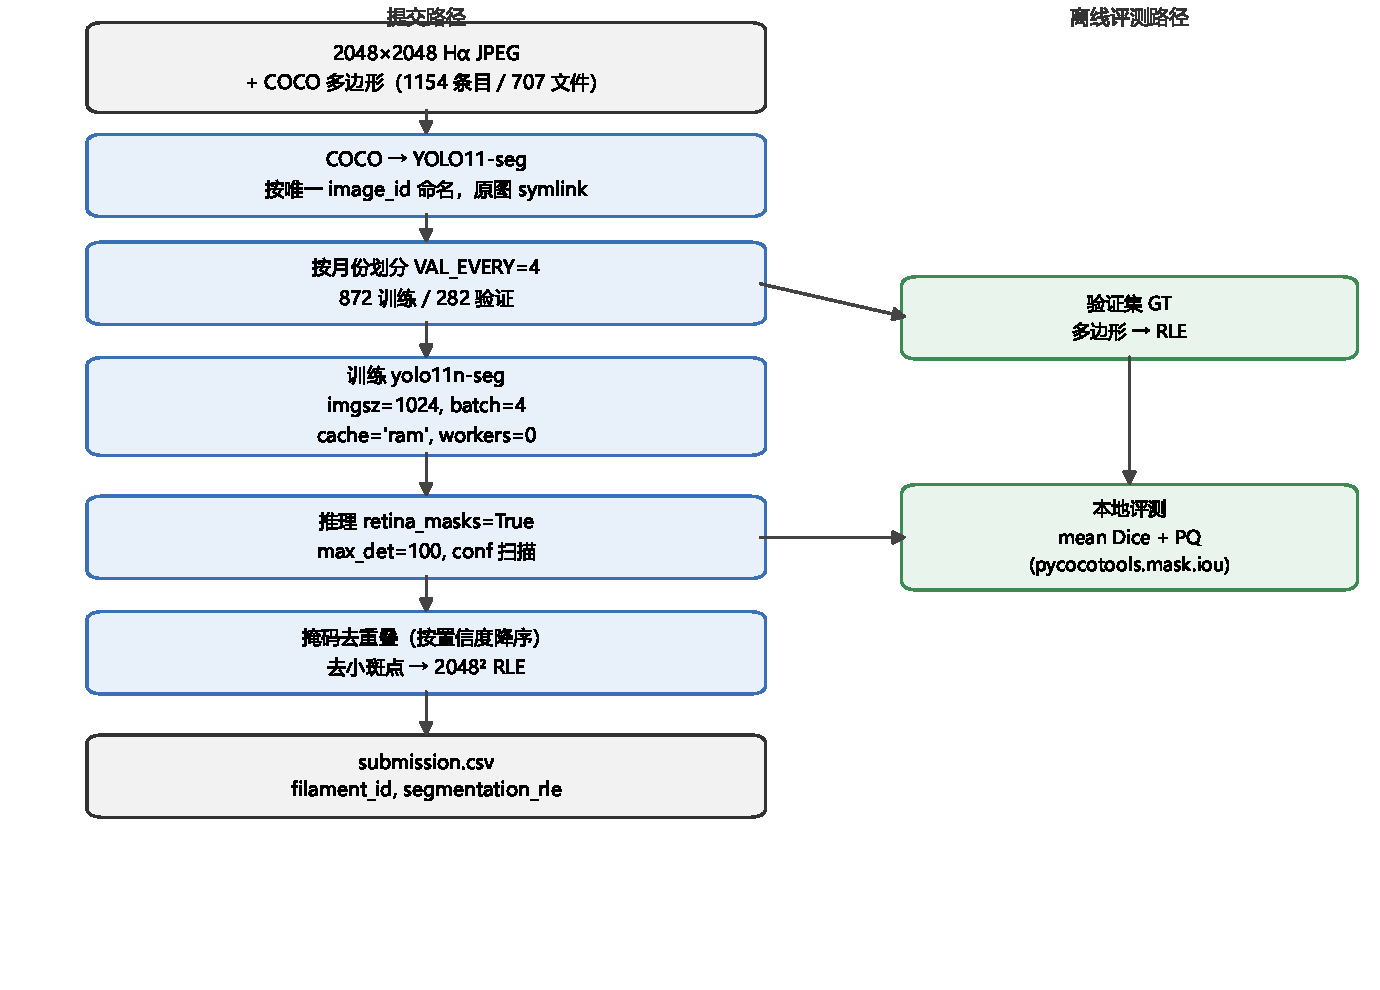
\includegraphics[width=0.92\textwidth]{fig_pipeline.pdf}
\caption{End-to-end pipeline. Left: the submission path, from the COCO file through the annotator-aware conversion and the month-grouped split to training and RLE submission. Right: the offline evaluation path, used only on the held-out month.}
\Description{Block diagram with a submission path on the left and an evaluation path on the right.}
\label{fig:pipeline}
\end{figure*}

% ====================================
% EVALUATION
% ====================================
\section{Evaluation}\label{sec:evaluation}

\subsection{Evaluation strategy and uncertainty}
We score predictions with the same matching semantics as the organisers' self-evaluation notebook \cite{pq}: a greedy one-to-one match at $\mathrm{IoU}>0.5$, and
\[
\mathrm{PQ}=\frac{\sum_{(\mathrm{y},\hat{\mathrm{y}})\in\mathrm{TP}}\mathrm{IoU}(\mathrm{y},\hat{\mathrm{y}})}{|\mathrm{TP}|+\tfrac12|\mathrm{FP}|+\tfrac12|\mathrm{FN}|}.
\]
Dice is computed per frame on the \emph{union} of that frame's masks, matching the leaderboard's use of \texttt{torchmetrics.segmentation.DiceScore}. All mask comparisons run on RLEs through \texttt{pycocotools.mask.iou}: a naive double loop over $2048^2$ boolean masks takes about an hour for $174$ frames, whereas the RLE version takes seconds.

Because a validation frame may carry one to three independent annotations, the ground truth itself is uncertain, and we can use that to measure our own noise floor. We re-score one fixed set of predictions (a single inference pass over the $174$ validation frames, $2520$ instances) under four ground-truth protocols (Table~\ref{tab:gt}), one of which is repeated five times with a randomly drawn annotator. The spread is $0.0021$ in global PQ and $0.0035$ in mean Dice. We therefore treat any PQ difference below $0.01$ as noise for the rest of this report.

\begin{table}[t]
\centering
\caption{Ablations, all on the same month-grouped validation split. Rows C and D share one set of weights and differ only in the confidence threshold.}
\Description{Table of four ablation runs with resolution, epochs, threshold, training time, and five metrics.}
\label{tab:ablation}
\small
\begin{tabular}{llrrrrr}
\hline
 & \textbf{imgsz} / ep / conf & \textbf{Dice} & \textbf{img-PQ} & \textbf{glob-PQ} & \textbf{tp/fp/fn} & \textbf{min} \\
\hline
A & 640 / 15 / 0.25 & 0.588 & 0.205 & 0.205 & 555/653/1539 & 9.9 \\
B & \textbf{1024} / 15 / 0.25 & 0.637 & \textbf{0.295} & \textbf{0.288} & 765/528/1329 & 13.4 \\
C & 1024 / 30 / 0.10 & \textbf{0.640} & 0.287 & 0.282 & 1030/1490/1064 & 32.8 \\
D & 1024 / 30 / \textbf{0.25} & 0.640 & 0.288 & 0.285 & 767/575/1327 & --- \\
\hline
\end{tabular}
\end{table}

\begin{table}[t]
\centering
\caption{Sensitivity to the ground-truth protocol. Same predictions, GT reassembled four ways. De-duplicating \emph{lowers} PQ.}
\Description{Table comparing four ground-truth protocols by Dice, PQ, and true positive, false positive and false negative counts.}
\label{tab:gt}
\small
\begin{tabular}{lrrrr}
\hline
\textbf{GT protocol} & \textbf{Dice} & \textbf{glob-PQ} & \textbf{fp} & \textbf{fn} \\
\hline
P0 union of all copies & \textbf{0.640} & \textbf{0.2816} & 1490 & 1064 \\
P1 first annotator only & 0.605 & 0.2622 & 1711 & 532 \\
P2 last annotator only & 0.616 & 0.2735 & 1678 & 475 \\
P3 random annotator ($\times5$) & 0.609 & $0.2663\pm0.0021$ & --- & --- \\
\hline
\end{tabular}
\end{table}

\subsection{Results}
\paragraph{Resolution is the only knob that clearly works.}
Downscaling to $640$ px costs $0.083$ global PQ ($0.288\to0.205$, a $29\%$ relative drop) and $0.049$ Dice. The gain from $1024$ px is almost entirely recall ($26.5\%\to36.5\%$; precision also rises, $45.9\%\to59.2\%$) for $3.5$ extra minutes of training. Filaments are thin: downscaling destroys them before the network ever sees them, so this is not a case of the model failing to \emph{interpret} the pixels but of the pixels being gone.

\paragraph{Doubling the training budget is a negative result.}
Going from $15$ to $30$ epochs raises every detection metric --- mask mAP50 $0.622\to0.638$, mask mAP50--95 $0.223\to0.236$, mask precision $0.61\to0.66$ --- but PQ does not follow ($0.288\to0.285$ at conf$=0.25$; $0.291\to0.282$ at conf$=0.10$), both inside the noise band. The mechanism is visible in the counts: longer training trades recall for precision ($0.592\to0.574$), and PQ penalises a miss and a false positive equally, so the trade cancels. Combined with the $\sim\!64\%$ redundancy of the training set, $15$ epochs are simply enough for a $2.8$M-parameter model.

\paragraph{Cutting false positives beats chasing recall.}
On validation, raising the threshold from $0.10$ to $0.25$ changes global PQ by only $+0.0029$ --- below our noise band --- but cuts false positives from $1490$ to $575$ and brings the total predicted instance count from $2520$ (roughly $2\times$ the $2094$ annotations) to $1342$ ($\approx$ the count of unique ground-truth instances). On the leaderboard the same change moved the public score from $0.21$ to $\mathbf{0.25}$ ($+19\%$ relative), with the submitted CSV shrinking from $2205$ to $1286$ rows. This is direct evidence that the competition metric is a composite that penalises fragmentation and over-merging rather than plain mean Dice: dropping $919$ low-scoring fragments was worth more than the recall it cost. We should be explicit about the limitation here --- the two submissions were produced by \emph{separately trained} models (the second by a full Commit run), so this is not a strictly controlled A/B; but $+0.04$ is an order of magnitude above the $0.0035$ Dice noise we measured.

\paragraph{Instance-level distributions.}
The rubric asks for three, all measured at the collecting threshold $\mathrm{conf}=0.10$. Figure~\ref{fig:dist} gives the first two. (1)~\textbf{Per-image Dice}: mean $0.640$, median $0.663$, $p_{10}$ $0.491$, $p_{90}$ $0.759$. Only one frame in $174$ fails outright, but \emph{not one frame exceeds $0.90$}, and $86\%$ land in $0.50$--$0.80$: the model is consistently mediocre-to-good and never collapses. (2)~\textbf{Matched-pair IoU}: mean $0.631$, median $0.622$, with $79\%$ of the $1030$ pairs between $0.50$ and $0.70$ and none above $0.90$. Matched masks barely clear the bar --- raising the PQ IoU threshold from $0.5$ to $0.7$ would discard roughly $79\%$ of the current true positives. (3)~\textbf{Prediction-to-GT relations} (Table~\ref{tab:rel}): $51.5\%$ of predictions match no ground-truth filament at all, and $35.5\%$ of filaments are claimed by no prediction. Fragmentation (one prediction claiming more than one filament) accounts for $13.9\%$ of predictions and merging (one filament claimed by more than one prediction) for $13.8\%$ of filaments --- almost equal, so no single failure mode dominates.

The three distributions explain the leaderboard result: \emph{half the predictions match nothing, and half the ones that do match barely clear the IoU bar}. The model over-produces low-tightness masks, and the $1297$ predictions that claim no ground truth are exactly what raising the threshold removed. Figure~\ref{fig:qual} shows both failure modes on real frames.

\begin{figure}[t]
\centering
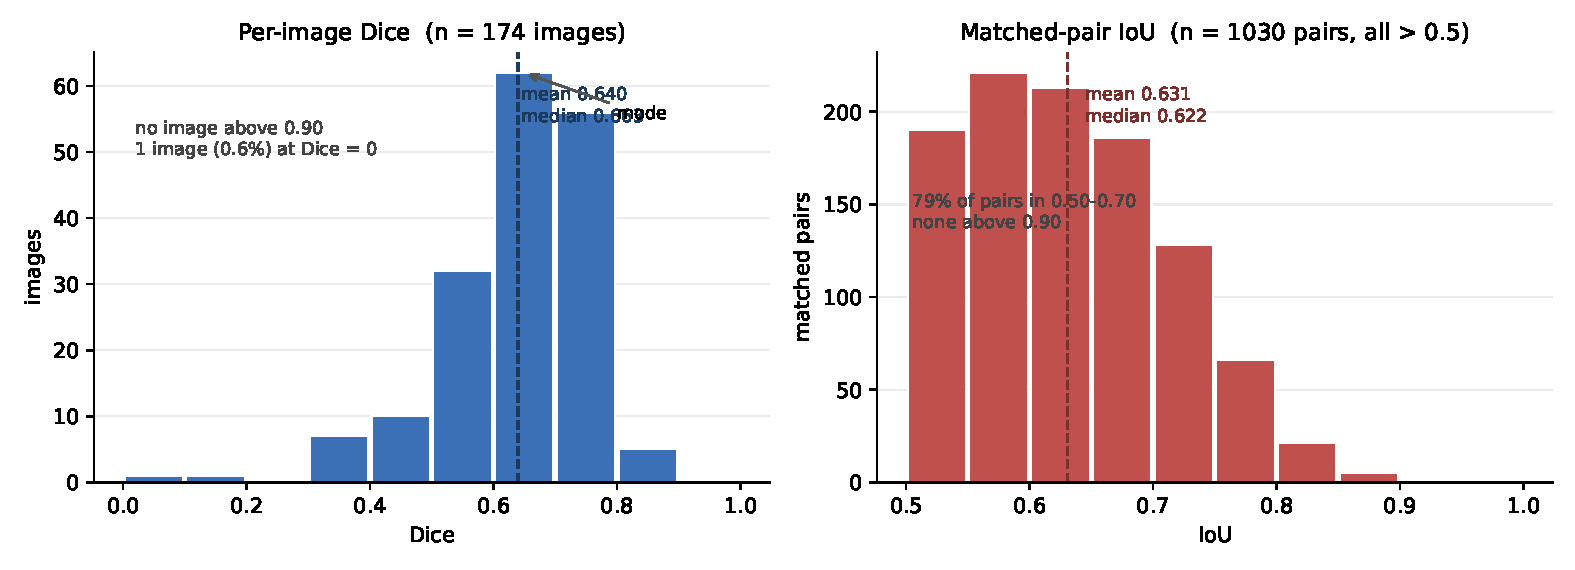
\includegraphics[width=0.98\columnwidth]{fig_distributions.pdf}
\caption{Per-image Dice (left) and matched-pair IoU (right), over $174$ validation frames and $1030$ matched pairs. Neither distribution reaches $0.90$.}
\Description{Two histograms, one of per-image Dice and one of matched-pair IoU.}
\label{fig:dist}
\end{figure}

\begin{table}[t]
\centering
\caption{Prediction-to-ground-truth relations. Left: how many predictions claim a given filament. Right: how many filaments a given prediction claims.}
\Description{Table of prediction and ground truth correspondence counts for k equal to zero, one, two and three or more.}
\label{tab:rel}
\small
\begin{tabular}{rrrr}
\hline
$k$ & \textbf{filaments with $k$ preds} & \textbf{preds claiming $k$ GT} \\
\hline
0 & 743 (35.5\%) & 1297 (51.5\%) \\
1 & 1062 & 872 \\
2 & 249 & 243 \\
$\geq3$ & 39 & 108 \\
\hline
\end{tabular}
\end{table}

\begin{figure}[t]
\centering
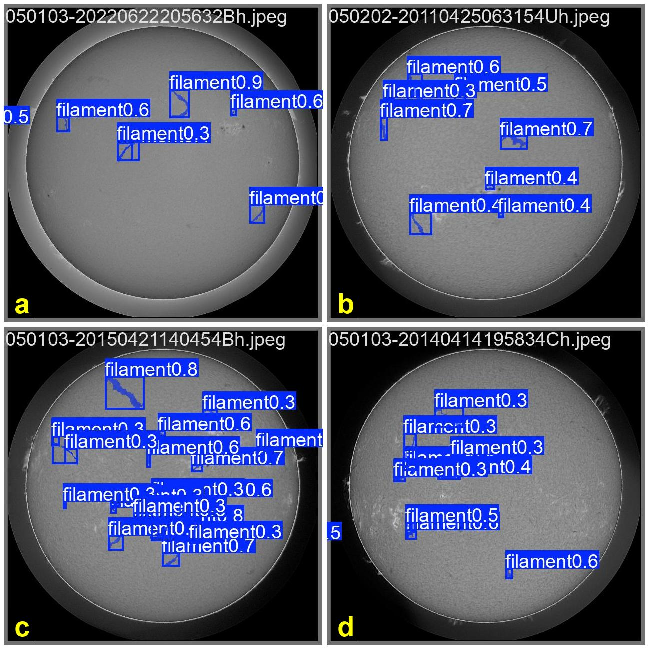
\includegraphics[width=0.98\columnwidth]{fig_qualitative.pdf}
\caption{Qualitative results on the validation month. Top row: filaments are separated and the mask outlines follow the structures. Bottom row: the two failure modes --- one large connected dark region cut into many overlapping boxes (fragmentation), and a diffuse region producing many low-confidence tinier instances while the real filament is never covered whole.}
\Description{Four H-alpha crops with predicted boxes and mask outlines; two successes on top, two failure cases below.}
\label{fig:qual}
\end{figure}

\subsection{Strengths, weaknesses, and next steps}
\textbf{Strengths.} The pipeline is small, cheap and fully reproducible on a free Kaggle notebook; the annotator-aware conversion and the month-grouped split remove two leaks that would otherwise inflate the validation numbers; and the evaluation is conservative --- we report uncertainty rather than point estimates, and we include a measurement that refuted one of our own hypotheses (Table~\ref{tab:gt}: we had inferred that merging duplicate annotations depressed PQ and estimated the corrected value at $\approx\!0.37$; de-duplicating instead \emph{lowers} PQ, because the annotators labelled complementary subsets and the union is the most complete ground truth).

\textbf{Weaknesses.} Recall is the binding constraint: at the threshold we submitted ($0.25$), $63\%$ of the $2094$ validation filaments are still missed; at $0.10$, where $51.5\%$ of predictions match no ground truth at all, half of them are still missed. Masks that do match are loose (IoU median $0.62$), which PQ punishes but Dice does not. All four ground-truth protocols stay below the organisers' $0.35$ bar, so the gap is not an artefact of the evaluation protocol.

\textbf{Next steps.} (1)~More pixels: train and infer at $1280$ or $1536$, which the resolution ablation says is the highest-yield direction. (2)~Inference better suited to elongated targets: sliding-window tiling and mask-level non-maximum suppression instead of a confidence threshold, which currently truncates candidates rather than merging them. (3)~The label side is untouched and costs no GPU time: the training set is $\sim\!64\%$ redundant, so multi-annotator consensus labels or down-weighting duplicate frames are cheap experiments. (4)~Swap the backbone for the larger \texttt{yolo26n-seg} variant named in the task sheet, which we did not have time to run.

% ====================================
% ACKNOWLEDGMENT
% ====================================
\section{Acknowledgment}\label{sec:acknowledgment}
% Do not change
The organization of the Filament Segmentation Challenge 2026 is partially supported by the U.S. National Science Foundation (NSF) under Grant No. 2209912 and 2433781, directorate for Computer and Information Science and Engineering (CSE), and Office of Advanced Cyberinfrastructure (OAC), and Grant No. 2511630, AST Division Of Astronomical Sciences and MPS Directorate for Mathematical and Physical Sciences. The Filament Segmentation Challenge 2026 is sponsored by the U.S. National Science Foundation (NSF) National Solar Observatory (NSO). This work utilizes GONG data obtained by the NSO Integrated Synoptic Program, managed by the National Solar Observatory, which is operated by the Association of Universities for Research in Astronomy (AURA), Inc. under a cooperative agreement with the National Science Foundation and with contribution from the National Oceanic and Atmospheric Administration. The GONG network of instruments is hosted by the Big Bear Solar Observatory, High Altitude Observatory, Learmonth Solar Observatory, Udaipur Solar Observatory, Instituto de Astrof\'isica de Canarias, and Cerro Tololo Interamerican Observatory.

\bibliographystyle{ACM-Reference-Format}
\bibliography{main}
\end{document}
